%% aps to author template--please use pdflatex to edit then to pdf--------------
\documentclass[A4,twoside,fontset=ubuntu,UTF8]{ctexart}
%\usepackage{slashbox}\usepackage{makecell}\usepackage{diagbox}\backslashbox
\usepackage{aappss}
\usepackage{subcaption}
%\usepackage{epstopdf}

\newcommand{\vx}{{\mathbf{x}}}
%\renewcommand\baselinestretch{1.235}\protect
\renewcommand\baselinestretch{2.0}\protect
\abovedisplayshortskip 0 pt plus 3pt
\belowdisplayshortskip 6 pt plus 2pt minus 2pt
\abovedisplayskip 6 pt plus 2pt minus 2pt
\belowdisplayskip 6 pt plus 2pt minus 2pt
% \info{2015}{64}{1}{01{}} \infodate{2015.0.0.}{2015.0.0.}
%=================== Text begin here ==============================
\begin{document}\apsname

\title{自动微分数值计算理论-地震波模拟为例 \fivestar}%{\cfundlink}

\author{刘金国$^{1)}$ \quad 许开来$^{2)}$}

\address{1)}{哈佛大学物理系, 坎布里奇 \quad 02138}
\address{2)}{斯坦佛大学, 斯坦佛 \quad 94305}

%\address{3)}{}

\abstract{自动微分是机器学习中核心的数值技术,它被用于高效,自动的对程序求导。
如今越来越多的物理学者意识到高效,自动的求导可以对很多物理问题的求解提供新的思路。
本文介绍自动微分技术相关的主要理论,并以地震波的模拟为例介绍它的应用。}

\keywords{自动微分,科学计算,编程语言}

% https://ufn.ru/en/pacs/all/
% 02.60.Pn numerical optimization
% 02.30.Jr Partial differential equations
\pacs{02.60.Pn, 02.30.Jr}

\cfund{}

\cmail{jinguoliu@g.harvard.edu \quad }

%\cmailddag{mail2}

%\mail{}{}\cmail \cmailddag

%\apscopyright \baselineskip=16.0pt plus.2pt minus.2pt
%\begin{multicols}{2}\sec
\vskip 0.55\baselineskip
\section{引~~~~言}
    自动微分是指自动获取一个目标计算机程序导数的技术。很多人了解它是因为它在机器学习中的成功应用,人们可以用它优化带有千亿参数的神经元网络~\cite{Rosset2019}。
与很多人印象不同的是,自动微分其实是个很古老的技术。
Nolan曾在他1953年的博士论文中就提出过~\cite{Nolan1953}自动化求导计算机程序的构想,
而最近十几年,自动微分在科学计算中的应用越来越广泛。
过去人们需要依赖手动推导求解导数,也因此限制了一个算法可处理问题的范围。一个典型的例子是变分蒙特卡洛算法。
过去,人们会将变分基态假设为Gutzwiller波函数~\cite{Gutzwiller1963}这样具有良好解析性质的函数。
直到2017年,Carleo等人~\cite{Carleo2017, Deng2017}把机器学习中的一些变分模型限制波尔兹曼机(RBM)带入到了大家的视野。由于RBM的解析性质很好,计算所需的求导过程可以通过解析推导,所以当时人们并没有强烈的利用计算机辅助求导的动机。
但受此启发,大家意识到不光是RBM这样解析性质好的函数,任何机器学习中的神经元网络也可以被用做波函数的猜测形式~\cite{Cai2018}。
而且如果可以用流行的机器学习框架,比如脸书公司开发的PyTorch和谷歌公司开发的TesnorFlow来编写生成波函数的代码,人们可以避免手动推导导数的麻烦,从而可以把波函数的表达变得更加自由。
而现在,随着人们对微分的认知更加深刻,波函数不光可以表达为以张量运算为主体的神经元网络,还可以是几乎任意的计算机程序。
%一段通用的代码总可以被分解成一些加减乘除这样的基础解析函数,知晓基础函数的自动微分规则,计算机可以通过链式法则用计算机推导出整个程序的导数。
    除了这个例子,科学家们利用方便的,自动化的计算机辅助求导还解决了很多包括量子模拟~\cite{Luo2019},张量网络~\cite{Liao2019},组合优化~\cite{Liu2020},海洋学~\cite{Heimbach2005}和地震学~\cite{Symes2007,Zhu2020}等领域中的问题。
甚至是一些非解析的蒙特卡洛抽样过程,人们也设计出了一些办法对其自动化的求导~\cite{Zhang2019}。

那物理学家们是否只需要奉行“拿来主义”,仅阅读机器学习库的文档,就可以很好的驾驭自动微分呢?
并不完全是的,当大家谈论自动微分的时候有“狭义”和“广义”之分,而主流机器学习库仅涵盖了前者。
这里狭义自动微分是指机器学习库中广泛应用的以张量为基本数据类型的自动微分。它通过对常用的函数族(矩阵乘法,卷积函数,relu函数等)手动定义导数后向传递的规则,并通过链式法则将它们连接起来得到程序的导数。
手动定义常用函数导数可以对函数有更加针对性的优化从而保证张量运算的性能,但缺点是,它往往无法满足科学计算的研究中对函数求导的多元化需求。有些时候人们可以通过手动添加一些求导规则来辅助求导,比如在张量网络等模拟中需要用到的复数奇异值分解函数~\cite{Wan2019,Liao2019}。
但是也有一些时候添加求导规则也无济于事,比如,严格对教化求解基态过程中用到的极大极小本正值求解器~\cite{Xie2020}和模拟变分量子算法中幺正量子线路的求导~\cite{Luo2019}的求导,前者涉及了无法表达为向量函数的稀疏矩阵的构造过程而后者涉及了利用可逆性回溯中间状态。
还有些时候手动定义的导数可能会出错,尤其是将定义在实数上的规则拓展到复数域的时候。比如奇异值分解函数的求导规则直到2019年,才有人意识到复数的求导规则中有一个规范不变性带来的一项被忽略了~\cite{Wan2019}。
而广义的自动微分没有这些问题,它微分规则定义在标量的最基础的运算之上,这些基础运算有限而且很难出错。
    一个很好的描述它与狭义自动微分区别的例子是,当将两个复数相加,广义的自动微分看到的是实部相加和虚部相加这两个操作,而狭义自动微分则需要推导适用于复变函数的Wirtinger导数~\cite{Hirose2003}。
但广义自动微分的强大威力同时也带来了一些问题,其中最核心的问题是它把机器学习中本身就存在的内存占用问题扩大了,
使得用户不得不直接或间接的面对这些问题。
为了让研究者们更好的利用广义自动微分解决物理中的实际问题,本文的向物理学家们介绍该领域中的几种核心概念以及它在微分模拟地震波传播过程中的应用。
章节\ref{sec:forwardbackward}~ 介绍了两种基本的自动微分模式,前向和后向自动微分。
章节\ref{sec:timespace}~ 介绍了基于检查点和可逆编程的两种广义后向自动微分的基础理论,尤其两者如何权衡程序的运行时间和空间。
章节\ref{sec:applications}~ 介绍了不同广义自动微分技术在微分地震波模拟过程中的应用。

\section{链式法则的两种传递方式}\label{sec:forwardbackward}

    在上世纪60年代,自动微分发展出了两种不同的实践,一种叫做前向传播(Forward propagation)~\cite{Wengert1964},一种叫做后向传播(Backward propagation)~\cite{Boltyanski1960}。


%为了直观的理解它们的不同,这里考虑一个计算过程 $f : \mathbb{R}^m \rightarrow \mathbb{R}^n$
%\begin{align*}
    %&\vx^1 = f_1(\vx^0)\\
    %&\vx^2 = f_2(\vx^1)\\
    %&\ldots\\
    %&\vx^L = f_L(\vx^{L-1})
%\end{align*}
%其中 $x^0\in R^m$, $x^L\in R^n$, $L$是计算的步骤数。
%这段程序的雅可比 (Jacobian) 矩阵$J_{ij} \equiv \frac{\partial x^L_i}{\partial x_j^0}$是一个$n\times m$的矩阵,其中$x_j^0$和$x_i^L$代表了输入和输出中的一个元素。
%前向自动微分的链式法则表述为$\frac{\partial \vx^k}{\partial x^0_j} = \frac{\partial \vx^k}{\partial \vx^{k-1}}\frac{\partial \vx^{k-1}}{\partial x^0_j}$,它计算了雅可比矩阵的第$j$列。后向自动微分的链式法则为$\frac{\partial \vx^L_i}{\partial x^{k-1}} = \frac{\partial \vx^L_i}{\partial \vx^{k}}\frac{\partial \vx^{k}}{\partial x^{k-1}}$,它计算了雅可比矩阵的第$i$行。
%在大多数应用中,计算一行雅可比矩阵比计算一列有用的多,因为
%后向自动微分的实现难度远高于前向自动微分,因为它的梯度计算方向和计算本身的方向相反,如何回溯中间状态成了一个核心的问题。

    \begin{figure}[t]
\centering
\begin{subfigure}[b]{0.32\textwidth}
    \centering
    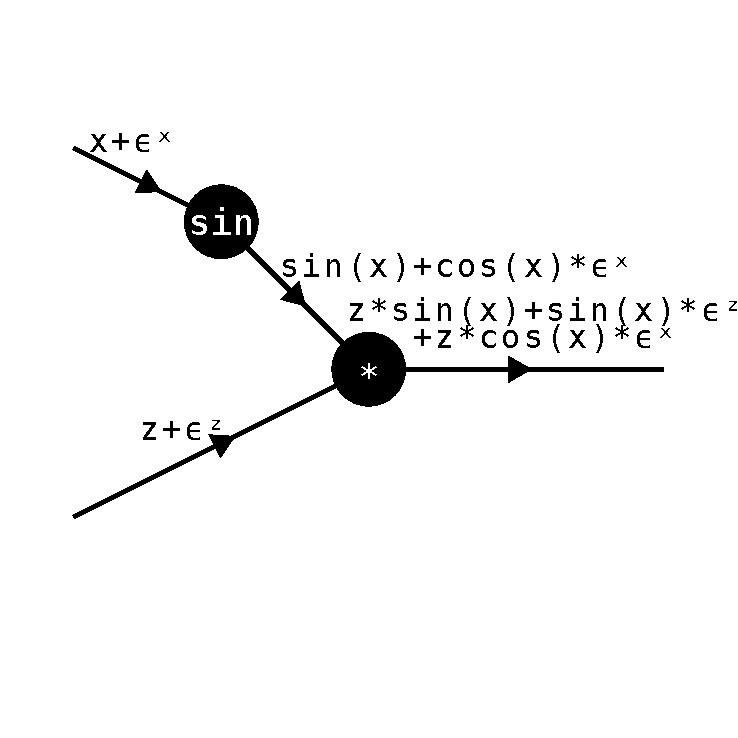
\includegraphics[width=\textwidth, trim={1cm 0 0cm 0}, clip]{./forwarddiff.pdf}
    \caption{前向自动微分}
\end{subfigure}
\begin{subfigure}[b]{0.32\textwidth}
    \centering
    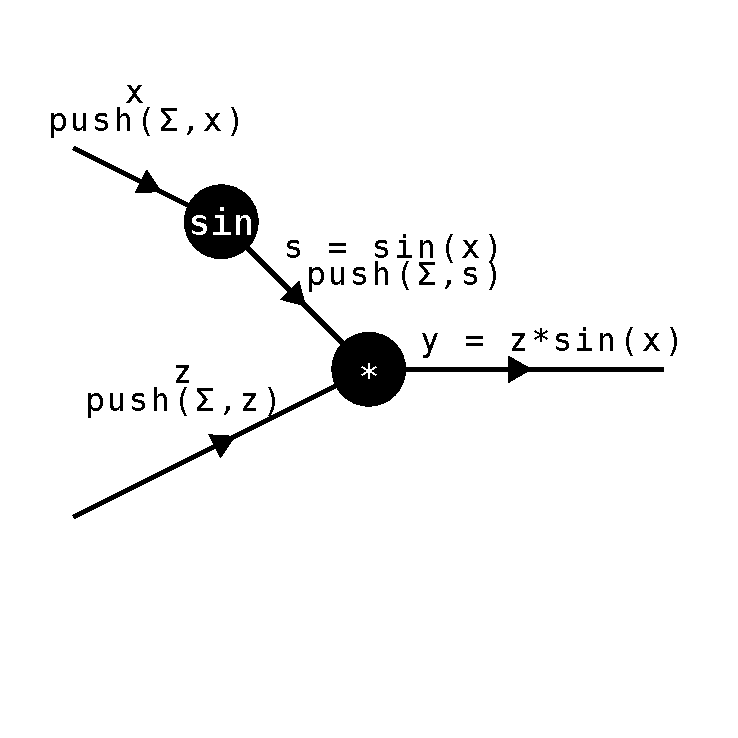
\includegraphics[width=\textwidth, trim={0 0 1cm 0}, clip]{./backward-forward.pdf}
    \caption{后向自动微分(1)}
\end{subfigure}
\begin{subfigure}[b]{0.32\textwidth}
    \centering
    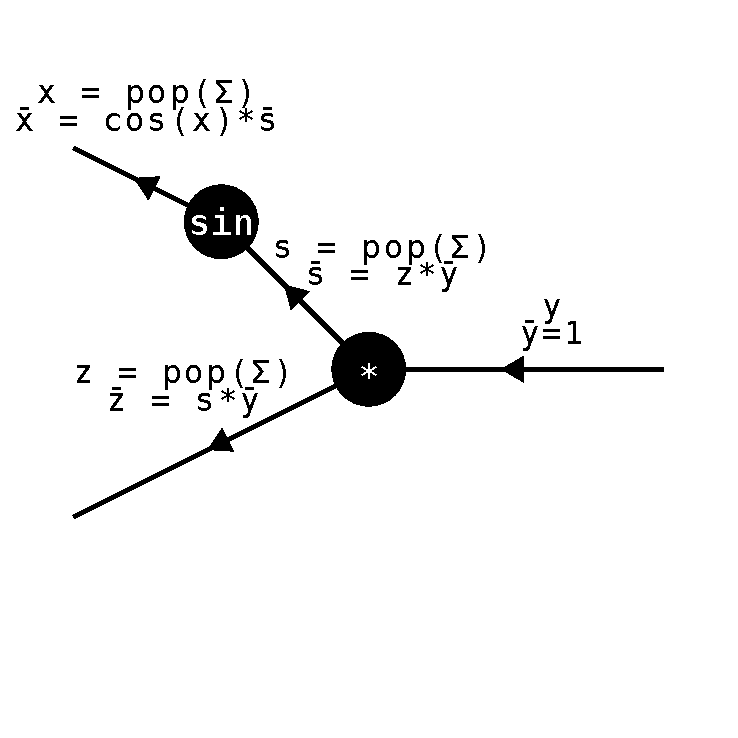
\includegraphics[width=\textwidth, trim={0 0 1cm 0}, clip]{./backward-backward.pdf}
    \caption{后向自动微分(2)}
\end{subfigure}
        \caption{利用自动微分计算对于计算过程$y = z \sin(x)$的导数$\overline{x}\equiv \frac{\partial y}{\partial x}$和$\overline{z}\equiv \frac{\partial y}{\partial z}$。\label{fig:autodifftypes}} 
\end{figure}

前向自动微分作用在标量上的梯度的第推公式为
\begin{align}
    f(x+\sum\limits^k_{i=1} y_i \epsilon_i) = f(x) + \frac{\partial f(x)}{\partial x} \sum\limits^k_{i=1}y_i\epsilon_i
\end{align}

其中,$\epsilon_i$正是我们高等数学中的“无穷小量”,而下标$i$代表它对应第$i$个变量。计算中我们只保留到一阶,因此它满足代数规则$\epsilon_i\epsilon_j = 0$。因此,实现一个前向自动微分本质就是实现一种携带无穷小量的特殊变量在函数作用下的变换。
前向自动微分的计算时间随着需求导的变量的数目线性增长。因为随着变量数目的增加,$\epsilon$的数目线性增加,函数的操作数也随之线性增加。
其中,$\epsilon_i$正是我们高等数学中的“无穷小量”,而下标$i$代表它对应第$i$个变量。计算中我们只保留到一阶,因此它满足代数规则$\epsilon_i\epsilon_j = 0$。因此,实现一个前向自动微分本质就是实现一种携带无穷小量的特殊变量在函数作用下的变换。
前向自动微分的计算时间随着需求导的变量的数目线性增长。因为随着变量数目的增加,$\epsilon$的数目线性增加,函数的操作数也随之线性增加。

后向自动微分作用在标量上的梯度的第推公式为
\begin{align}
    \overline{x} = \frac{\partial f(x)}{\partial x}\overline{y}
\end{align}
其中,$\overline{x}\equiv \frac{\partial \mathcal{L}}{\partial x}$为变量$x$的梯度,这个定义同时隐含了程序最终会输出一个标量$\mathcal{L}$作为损失函数。值得注意的是,为了计算$\frac{\partial f(x)}{\partial x}$,我们往往需要知道额外的一些信息,比如$x$的数值。但是在后向传播过程中,知道中间变量数值并非易事,我们或是把需要的变量放入一个全局的堆栈,或是利用可逆编程写可逆的代码并通过反向执行来获取中间变量数值。


\section{时间与空间的权衡}\label{sec:timespace}

引言中,我们提到后向自动微分有一个无法避免的共同问题,那就是如何回溯中间状态。
回溯中间状态最简单的做法是,记录程序的初始状态,当需要获取第$k$个计算状态$s_k$,程序从初始状态$s_0$开始进行$k$步运算。这么做缺点明显,那么就是需要$O(T^2)$的运行时间。
当磁盘空间充裕,程序可以在每一步都进行状态拷贝,虽然有$O(T)$的额外空间开销,但是没有额外的用于运算时间。
但很多实践中,不管是$O(T^2)$的时间开销或者是$O(T)$的空间开销都无法被接受,人们更需要的是一个均衡的计算时间和计算空间的方案。
    在程序运行的何时,何处进行状态拷贝,成为了检查点方案的问题核心。最优的关于时间和空间交换的检查点方案在1992年被Griewank~\cite{Griewank1992}提出,它是很多广义自动微分框架的基础。算法的梗概如图\ref{fig:tradeoff} (a)所示,
    算法把计算过程分割成$d$个区块,并记录每个区块的开始状态,每个区块的大小由函数$\eta(\tau, \delta)$决定,其中$\delta=1\ldots d$为从末尾开始数的区块的指标,$\tau = 1\ldots t$是一个超参数并被初始化为$t$。
最后的区块最小,因此可以用上述$O(T^2)$的算法来获取中间状态,回溯完最后一个区块后,程序释放最后一个区块开始处被缓存的状态。
于是在接下来计算倒数第二个区块的过程中,我们可以在这个计算过程中多缓存一个状态而不增加最大内存开销。类似的,倒数第$\delta$个分块可以使用的额外状态缓存数为$\delta-1$。
对每个分开递归的调用这个算法$t$次,每次将$\tau\leftarrow \tau-1$,最后得到的分块的大小为$1$。整个算法的时间和空间开销的关系是
\begin{align}
    T_c = tT, S_c = dS,
\end{align}
其中,$T = \eta(t, d)$是初始计算时间。选择适当的$t$或者$d$,在时间和空间维度上的额外复杂度可以都是$\log(T)$。

回溯中间状态还有另一种做法,那就是可逆计算。可逆计算的代码天然可以被回溯,但是也会因此带来额外的时间或空间的开销。由于直接赋值在可逆计算中不被允许,最直接的将不可逆代码变成可逆代码的方法是先分配内存,用累加的方式,
\begin{align}
    &\vx^1 \ldots \vx^L \leftarrow 0\\
    &\vx^1 \mathrel{+}= f_1(\vx^0)\\
    &\vx^2 \mathrel{+}= f_1(\vx^1)\\
    &\ldots\\
    &\vx^L \mathrel{+}= f_1(\vx^{L-1})
\end{align}

%On the other side, the optimal time-space trade-off scheme in reverse computing is the Bennett's algorithm illustrated in \Fig{fig:tradeoff} (b). It evenly \textbf{evenly} partition the program into $k$ sectors. The program marches forward ($P$ process) for $k$ steps to obtain the final state $s_{k+1}$, then backward ($Q$ process) from the $k-1$th step to erase the states in between $s_{1<i<k}$. This process is also called the \textit{compute-copy-uncompute} process. Recursively apply the compute-copy-uncompute process for each sector until each $P/Q$ process contains only one unit computation. the time and space complexities are
\begin{align}\label{eq:rev}
    T_r = T\left(\frac{T}{S}\right)^{\frac{\ln(2-(1/k))}{\ln k}}, S_r = \frac{k-1}{\ln k}S\log\frac{T}{S}.
\end{align}
%Here, the overhead in time is polynomial, which is worse than the treeverse algorithm. The treeverse like partition does not apply here because the first sweep to create initial checkpoints without introducing any space overheads is not possible in reversible computing. The pseudo-code of Bennett's time-space trade-off algorithm is shown in \Lst{lst:bennett}.

\begin{figure}
    \centerline{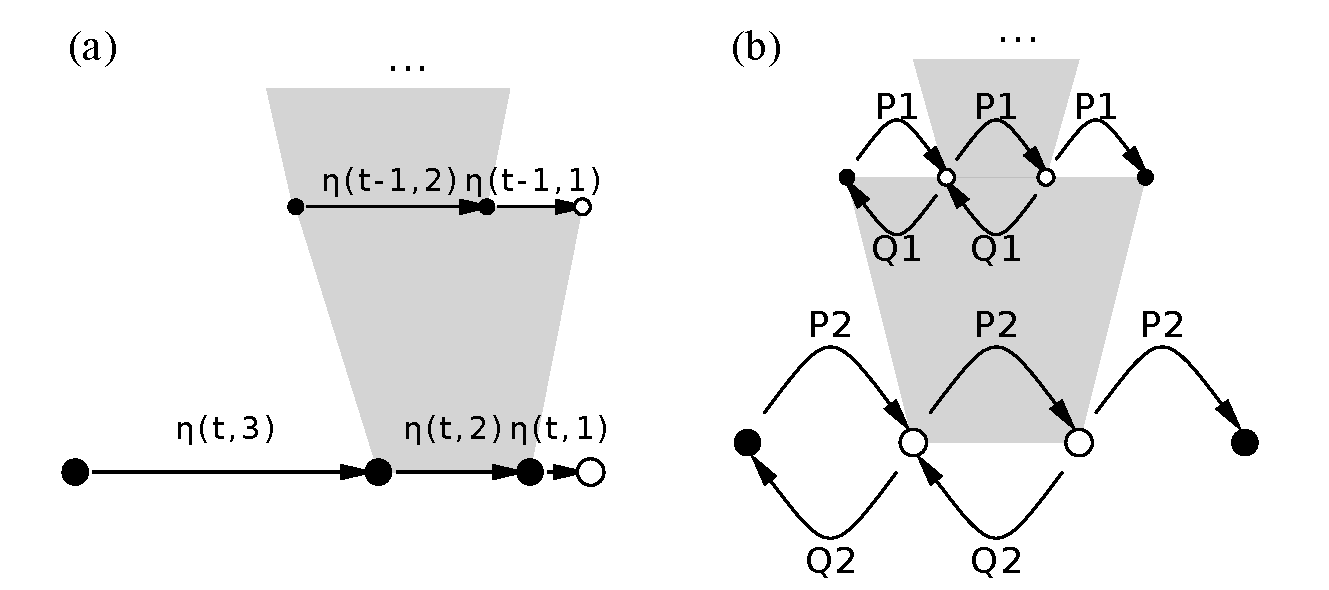
\includegraphics[width=0.88\columnwidth,trim={0 0cm 0 0cm},clip]{tradeoff.pdf}}
    \caption{(a) 广义自动微分中常见的Treeverse算法~\cite{Griewank1992},其中$\eta(\tau, \delta) \equiv \left(\begin{matrix} \tau + \delta \\ \delta \end{matrix}\right)=\frac{(\tau+\delta)!}{\tau!\delta!}$。(b) 可逆计算时空交换的Bennett算法。~\cite{Bennett1973,Levine1990} 其中,$P$和$Q$分别代表了计算和反计算。它的伪代码是代码块\ref{lst:bennett}。}\label{fig:tradeoff}
\end{figure}


\begin{figure}[t]
\centering
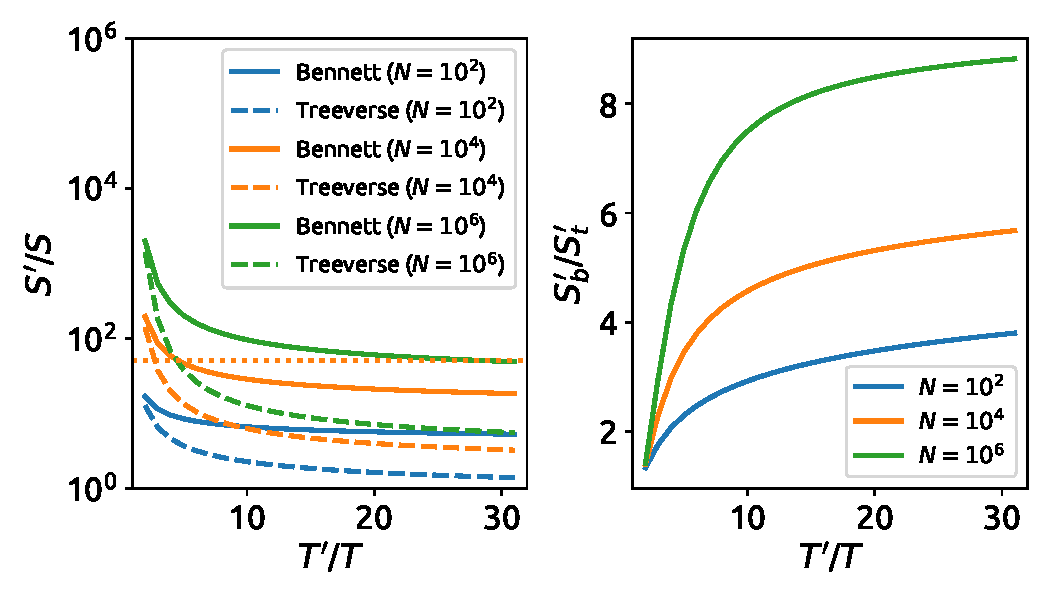
\includegraphics[width=0.8\columnwidth]{./fig1.pdf}
    \caption{为了回溯中间状态,时间和空间在两种最优时间-空间交换策略下的关系。(a) 固定横轴为状态回溯的计算时间与原函数计算时间的比值,对比再允许固定时间开销下,内存的额外开销。其中Bennett算法代表了可逆计算下的最优策略,而Treeverse则是传统计算允许的最优策略。(b) 对比Bennett算法与Treeverse算法空间开销的比值。\label{fig:timespace}} 
\end{figure}


\section{自动微分在物理中的应用}\label{sec:applications}
\vskip 1.55\baselineskip
\subsection{地震波的模拟}
后来在地震学的模拟中,它被用来微分地震波传播的过程~\cite{Symes2007}。

\vskip 1.55\baselineskip
\subsection{热带(Tropical)张量网络求解自旋玻璃最优构型}
热带张量网络是张量网络的一个特别的应用,它重新定义了张量中基础元素的代数为
\begin{eqnarray}
x \oplus y  = \max(x, y),\,\,\,\,\,\,\,\,\,\,\,\, \,\,\,\,
x \odot y   =  x + y. \label{eq:max-sum-alg}
\end{eqnarray}
\begin{figure}[t]
\centering
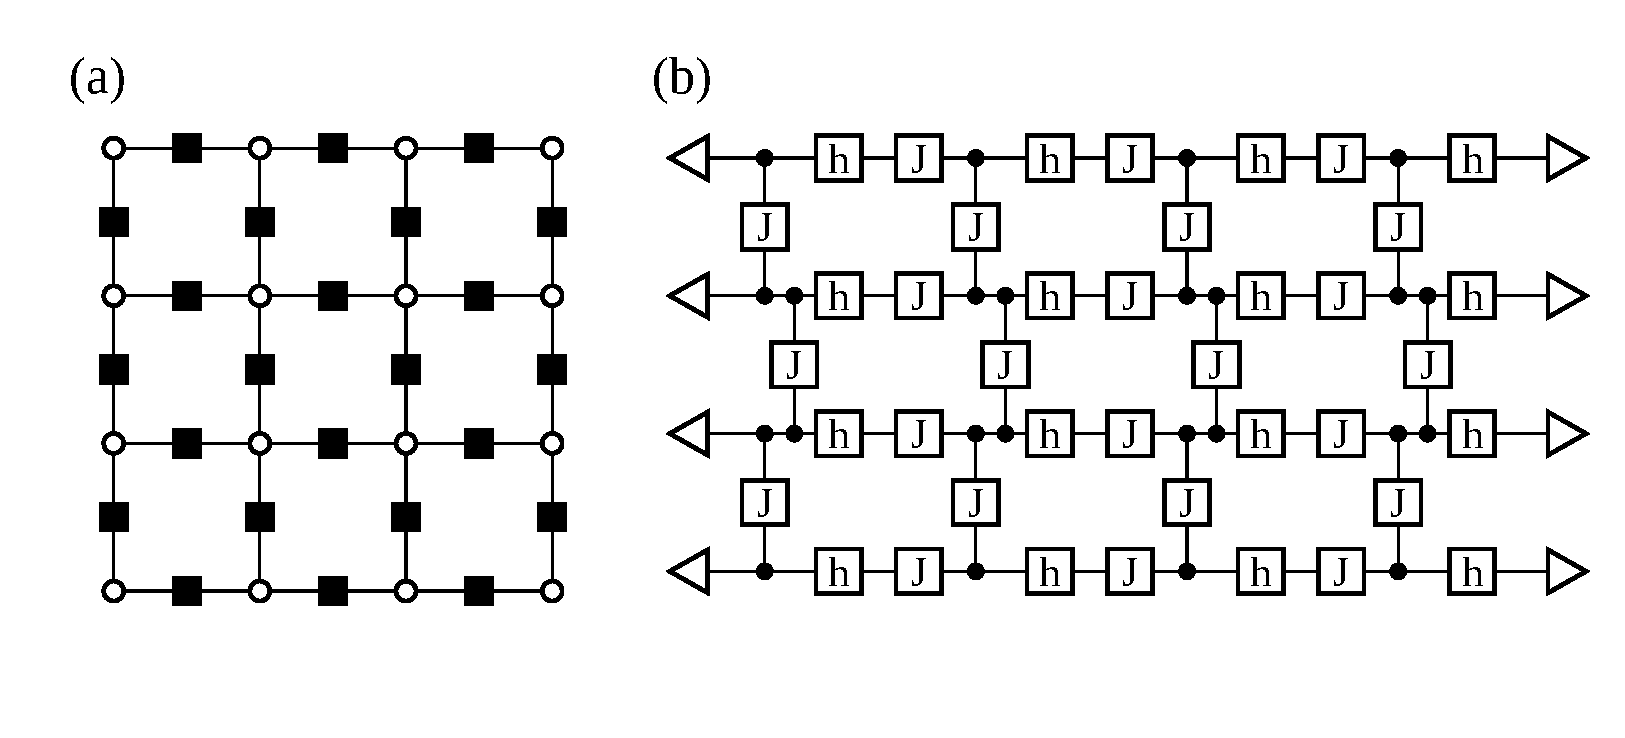
\includegraphics[width=\columnwidth]{./transform12.pdf}
    \caption{正方晶格上的自旋玻璃问题,(a)对应的热带张量网络表示。(b)对应的“量子线路”表示。\label{fig:performance}} 
\end{figure}
如果我们将张量中的元素定义为自旋玻璃的耦合强度,我们就可以通过收缩这个张量结构得到自旋玻璃的最优构型。
这个最优构型的能量表达式为
\begin{equation}
    E(\{\sigma\}) = \max\limits_{\sigma}-\sum_{i < j }J_{ij} \sigma_i \sigma_j  - \sum_i h_i \sigma_i,
\label{eq:spinglassopt}
\end{equation}
    因此对它的微分就是。
但是作了这样的替换,张量收缩的微分规则就发生了变换。

\section{结~~~~论}

\section*{致谢}

感谢北京大学力学系某某教授和某某博士以及某某的讨论.


\section*{附录A1}

标题排列和编号方式为A1, A2, A3.

\section*{附录A2}
%
%text text
%
%\section*{附录B1}
%%\section*{附录B2}
%
%text text
%
%\section*{致谢}
%
%text text

\bigskip
%\begin{footnotesize}

\bibliographystyle{apsrev4-1}
\bibliography{refs}

\newpage

\title{English Title $^{\ast}$}%{\efundlink}

\efund{Project supported by the State Key Development Program for Basic Research of China (Grant No. 2011CB00000), the National Natural Science Foundation of China (Grant Nos. 123456, 567890), and the National High Technology Research and Development Program of China (Grant No. 2011AA06Z000). \\}


\author{Guan Yun-Chang$^{1)2)}$ \quad  Liu Bei$^{1)\dag}$ \quad  Zhuge Liang$^{2)}$}

\email{aaa@bbb.ccc  }
%\email \emailddag


\eaddress{1)}{State Key Laboratory of Quantum Optics and Quantum Optics  Devices,
Institute of Opto-Electronics, Shanxi University, Taiyuan 030006, China}

\eaddress{2)}{Department of Physics, Tsinghua University, Beijing 100084, China}

\eabstract{}

\small  To determine the probe made of amino acids arranged in a linear chain and joined together by peptide bonds between the carboxyl and amino groups of adjacent amino acid residues. The sequence of amino acids in a protein is defined by a gene and encoded in the genetic code. This can happen either
before the protein is used in the cell, or as part of control mechanisms.

\ekeywords{Keyword1, Keyword2, Keyword3, Keyword4 \\}

\epacs{02.10.Yn, 33.15.Vb, 98.52.Cf, 78.47.dc}

\end{document}
